\chapter{Implementation}
\label{cha:implementation}

In this chapter we explain briefly the techniques used to implement both the front-end and the back-end.
We first elaborate on the different roles existing in the front-end:

\section{Frond-end}

\textbf{IDE}: Visual Studio code\\
\textbf{Language}: React\\
\textbf{Libraries used}:
\begin{itemize}
    \item React-router-dom
    \item Receiver mail must be a registered user
\end{itemize}


\subsection{Home Page}
\textbf{http://localhost:3000/\#/}\\*
\\*
After a successful log in all roles (postmen, company, customer) will be redirected to the same home page.
This home page presents a table containing a minimized version of the package data as per the role.
The user can here get a brieg=f information regarding the packages under his/her ID and its corresponding status.\\*
Algorithm:
\begin{enumerate}
    \item Extracting the user role. Each user as part of the Google authentication has a role type stored in the local database upon first time log in.(postman, customer, company) 
    \item \textbf{http://localhost:8000/packages/user/}  get request, before the component is mounted : upload package and information. The information will then be displayed as a table.
\end{enumerate}



\subsection{customer}
Libraries used:
\begin{itemize}
\item rc-slider - for creating the temperature slide bar 
\item react-horizontal-timeline - for the time line view
\item redux-form - for the registration form
\end{itemize}

The customer role refers to any individual who sends a package through the system.
The customer has the following abilities:

\begin{itemize}
    \item Register a package
    \item Delete a package
    \item view a package detail  
    \item view time line of the package
\end{itemize}


\subsubsection{Register a package}
\textbf{http://localhost:3000/##/packages/registerPackage}\\
\\*
The register package process is divided into two components:
\begin{itemize}
\item RegisterPackage.js - view 
\item UserSpace.js - controller 
\end{itemize}


\begin{figure}[!ht]
	\centering
	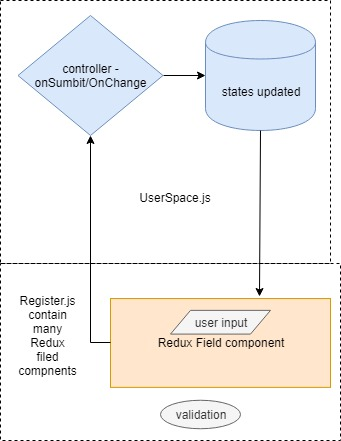
\includegraphics[width=0.5\textwidth]{images/register.jpg}
	\caption{register package process, component diagram}
	\label{fig:}
\end{figure}


The component RegisterPackage is an assembly of Redux <Field> component and React input.
for each input field the user enters, the specific page is rendered and the consequent state is updated.
The form contain the following validation:
\begin{itemize}
\item No text input field can be left empty 
\item Receiver mail must be a registered user
\end{itemize}
i.e without standing in the form requirement, the user can not press the submit button.

When registering a package, a sensor data may be provided by clicking on the corresponding check box. It is important to mention that not every package needs to have sensor data.\\*
Algorithm:
\begin{enumerate}
  \item \textbf{http://localhost:8000/address} post request,enters the address and returns an ID for each address provided.
    \begin{enumerate}
        \item \textbf {http://localhost:8000/packages}  post request, enters the package to the packages table, returns a package ID procided an address ID as input
        \begin{enumerate}
        \item \textbf {http://localhost:8000/OrderSensors}  post request, enters the sensor information (if exists)  into the sensors table, returns a sensor ID provided a package ID as input
        \end{enumerate}
    \item \textbf {http://localhost:8000/OrderHistory}  post request, enters the action(registration) as part of the order history to be used later on as part of the time line display - If and only if a package and sensor id is provided\\
    \end{enumerate}
\end{enumerate}

Only after fetching the data successfull from the database the page content will be replaced to a "package has been registered" message.


\subsubsection{Cancel package}
\textbf{http://localhost:3000/#/packages/active}\\

The feature cancel package allows the user to cancel a package.
After pressing the navigation bar with the "delete package" option, the user will be directed to the Active.js component.\newline
The user will be shown a data-minimized table only with packages in a "registered" status, \textbf{any other package which has been dispatched already cannot be canceled}.\newline
From the system perspective while the package is being canceled, the data is not deleted from storage,it will only be marked as canceled.\\*
Algorithm:
\begin{enumerate}
  \item \textbf{http://localhost:8000/packages/user/}  get request, before component is mounted : upload all packages with "registered" status,
  \item If user deletes a pacakge:
  \begin{enumerate}
      \item \textbf {http://localhost:8000/packages/:id}  put request. Change the specific package to "canceled" status.
      \item \textbf {http://localhost:8000/OrderHistory}  post request. Update the time line, add an event to Orderhistory table.
\end{enumerate}
\end{enumerate}


\subsubsection{Detailed package view}
\textbf{http://localhost:3000/##/package/ID}\\
\\*
The feature allows the user to view extensively the package information and the package time line.
After choosing the specific package ID in the home page,the user will be redirected/routed to this component.This ID will be transfer ed as a property from the home page to the Detailed.js component. 
In addition to the package data which was provided during the registration, the table also displays the current status of the package and the condition of the package.i.e if the user requests for a sensor, the table will display the number of events where the condition was not satisfied.
The sensor data will be only present if the user registers a sensor to the package.\\*
Algorithm:
\begin{enumerate}
  \item \textbf{http://localhost:8000/packages/details/id}  get request, before component is mounted : uploads the package information. The information will be displayed in the form of a table
  \item \textbf{http://localhost:8000/packages/orderHistory/id}  get request, before component is mounted : uploads the package history.The history willthen be sent to the Timeline.js component as a property.
  \begin{enumerate}
      \item Timeline.js uses the npm package "react-horizontal-timeline" to display the package in the form of a time line.
      the time line displays the status of the package, the company and postman name related to the package at that instance.
    \end{enumerate}
\end{enumerate}


\subsection{Company}

Company user in the system will be able to do the following activities:-

\begin{itemize}
\item \textbf{View package pickup request sent by customer to the particular company.}
When customer registers package, package is registered to DC3 database with registered status. Company will see assigned package on the system filtered by status.
\item \textbf{Accept package pickup request from customer my assigning to the postman under the company.}
The registered package is accepted by company by assigning to available postman of the company for pickup from the customer location. Company does this by clicking Assign button which calls assign.js. Company has to enter the email address of postman on the form and click the button. After the package is assigned to particular postman the status of package will be change to Transit in the database. There is Assign Package Sub-menu under User Management for the package assign function
\item \textbf{Upgrade users to postman or another company user of the same company.}
Company can upgrade registered user to postman or to another company user of the same company by entering email address. For the upgrade function to be applied to particular user. The user has to register themselves as customer first. There is sub menu on sidebar under User Management for this function. UpgradeUser.js is used for this functionality.
\item \textbf{View tracking history of packages under the company.}
When company user login to the system, in the dashboard there will be all the list of packages that have been under the particular company. By clicking on order ID on the leftmost side it takes to detail page of particular company with tracking history of the packages shown as timeline.
\item \textbf{View user list of own company and change their role to available roles in the system.}
Company can see user list of and upgrade individual to postman or another company user as discussed above.
\item \textbf{Create incident for the packages}
Company can create incident for the particular packages if any alteration on the condition is noticed. For this purpose a separate menu is established on sidebar as Incident Management. Incident are created by putting Package ID and incident description under Create Incident sub-menu. 
\item \textbf{View and resolve the incident of particular packages.}
Company can view and resolve the incident for packages if those incident has been resolved. For this company has to click resolve incident button on the incident list displayed in Incidents sub-menu under Incident Management menu.
\end{itemize}


\subsection{Postman}

\begin{figure}[htp]
    \centering
    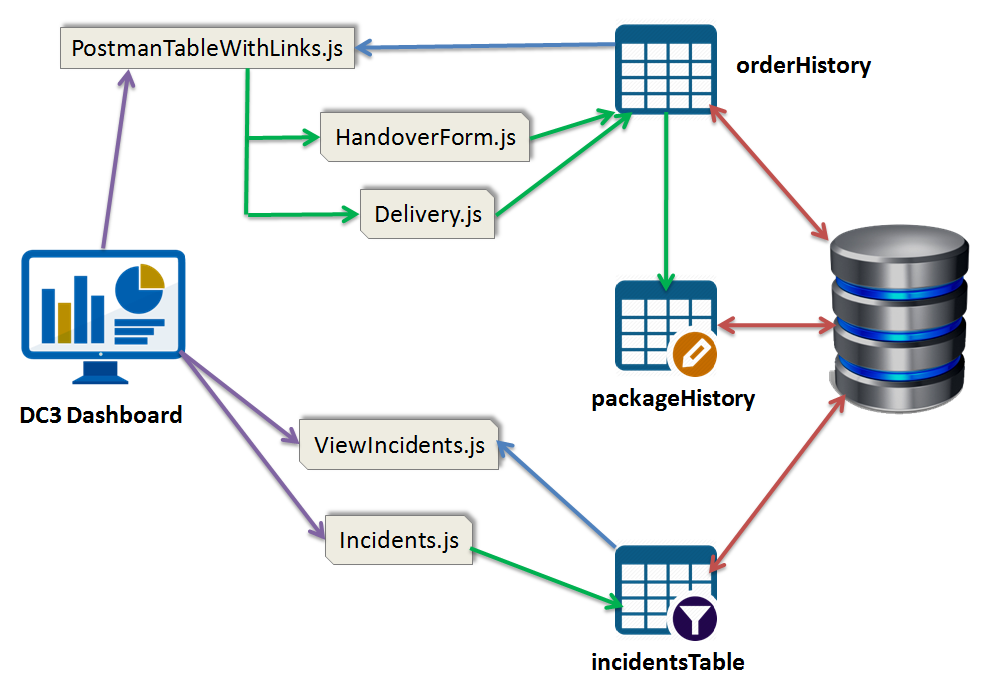
\includegraphics[width=4 cm]{images/snet/DC3 Postman.png}
    \caption{DC3 Postman}
    \label{fig:}
\end{figure}

\textbf{Overview of the functionality:}

Postman user in the system will be able to do the following activities:-
\begin{itemize}
\item {\textbf{View all the packages that have been assigned to him: }}(PostmanTableWithLinks.js) When the Company user assigns a package (PackageId) to a particular postman (PostmanId) then a relevant record is created into the table orderHistory. All the packages that are assigned to the current user are fetched using http://localhost:8000/orderHistory

\item \textbf{View the information about the package such as pickup address, drop address, status etc:} The table orderHistory contains columns that hold the relevant data of the package required for the postman to identify every package.
\item \textbf{Able to change the status of the package as Delivered once the actual delivery has been made:} whenever a postman physically delivers the package to the recipient at the respective Drop Address, then he is able to press the button 'Deliver' that invokes the function to setthe status of the Package as 'Delivered' and enter a new row in the packageHistory table only to denote that the package is now counted as one of the delivered packages.
\item \textbf{Able to Handover the package by assigning it to another Postman and change the status accordingly: }whenever a postman reaches an intermediate point in the route of the package where he has to hand it over to another postman, then the 'Handover' button is used to redirect to another component HandoverForm.js where the user id of the receiving postman needs to be entered. This functionality allows one postman to assign a package to nother postman by changing the 'AssignedTo' data in the relevant table. After this subroutine is invoked the handed over parcel  starts to appear in the dashboard of the receiving postman.
\item \textbf{Able to raise Incident whenever there is any violation of policies:} A postman to who the package has been assigned or handed over is able to judge the condition of the package and raise an incident mentioning the details of the package and the nature of violation also mentioning its current condition using the form created in the Incident.js component.
\item \textbf{View the Incidents that have been raised in the past: }Under the heading 'Incident Management' there is a link 'View Incidents' that redirects to ViewIncidents.js component that pulls data from the Incidents table and allows the Postman to see the relevant list of Incidents raised by or against him that have not yet been resolved.
\end{itemize}


\subsection{Integration, Routing and Common web pages }

\subsubsection{Integration}
As per the aforementioned statements in the earlier section, we have developed a Single Page Application (SPA) which holds together or integrates our complete application. In the application we render only one main page with a constant navigation bar and a side bar which provides usage features present on the navigation bar and the side bar based on authorization with respect to the role being assigned to the user.
The main page is further made of the header component, the footer component and the main component. The header component contains mainly the navigation bar which includes brand logo and a common sign out option for all users and the footer component contains a common footer that is rendered at all times in the page.
Further the main component inside the main page consists of the side bar and the user information.This component is rendered always as part of the SPA.The user information is itself a smaller component that displays the name, type of customer and a display picture of the user. The side bar consists of options that differ for each user based on the role assigned to the user. The main challenge here was to render the specific options with respect to role and all the common options that needed to be available for all the users in common.

The navigation bar and the side bar in our application is developed using the Bootstrap framework. It contains the duo of React and Bootstrap.The "NavBar" component was primarily used to develop the navigation bar and the side bar. Many features to toggle between entities or collapsing based on conditions were made use of from the "react-bootstrap" library with the help of some components like "Nav", "NavItem", "NavDropdown", "FormGroup", "FormControl" which were made use for better structuring of web page.

\textbf{Libraries used}:
\begin{itemize}
    \item react-bootstrap
    \item react-redux
\end{itemize}

\subsubsection{Routing}

Having our application as a single page application, it is vital to route through to correct pages or render correct components on click of routing links or buttons.
Having said that, all of our routing in the application takes place by clicking on options being rendered on the side bar or the navigation bar. As mentioned in the previous section authorization based rendering of features were first done post this on click of an option we routed the exact path of the component which was to be rendered upon clicking the link or the button. By using this mechanism we made sure a single main page was rendered upon log in and routed to respective components based on the specified routes.

To achieve this feature comprehensively, we used the "Route", "Router" and "withRouter" components from the library "react-router-dom" where we specified the exact path of the component by using the "Route exact path" or "Route path" features from the above mentioned components. Using these components from the libraries not only made the routing precise but also helped us to keep the code organized and well structured.

\textbf{Libraries used}:
\begin{itemize}
    \item react-router-dom
    \item react-redux
\end{itemize}

\subsubsection{Common web pages}
DC3 web application has three main roles or personas and each of which have different features provided in the application based on the type of role the user is assigned to. But some features in the applications are common for all of the users. For these features rather than developing repetitive pieces of code to provide the same, we developed a single component for the feature and reused the component as per requirement. 
The landing page is a common web page that all the users irrespective of the role can access. Apart from that the major functionality like the home page or the default page post log in is  common for the three kind of users was developed once and reused in different parts of the application where it portrays package history information on a minimized scale. It is filtered based on most recent and to a limited number of packages being displayed in a table format.

Another functionality that was common upon log in for all users was the incident management section. In the application, be it a customer, a company representative or a postman , all of them need to have authorization to create an incident with respect to a package. hence a set of common components like "create incident" , "view incident" was developed that could be reused.
On click of the "create incident" , the web page displays the incidents raised by the user with respect to the customer,  displays the incidents raised by the postman and the packages assigned to the postman with respect to the postman role and finally displays all incidents of packages that have been assigned to the specific company with respect to a company user.

\begin{enumerate}
  \item \textbf{http://localhost:8000/Incidents}  get request helps to retrieve the specific incidents with respect to the user based on roles.
  \item \textbf{http://localhost:8000/Incidents} put request helps to add an incident to the Incident table.
  \item \textbf{http://localhost:8000/Incidents} update request helps to resolve the incident by changing the status of the incident in the Incident table and will not be retrieved through a get request post status change.
\end{enumerate}

The component RaiseIncident is has a combination of "Redux" component, built using a "form" component.
for each input field the user enters, the specific page is rendered and the consequent state is updated.
The form contains the following validation:
\begin{itemize}
\item No text input field can be left empty,
\end{itemize}
which clearly notifies that without standing in the form requirement, the user can not press the create incident button to submit the form.

\textbf{Libraries used}:
\begin{itemize}
    \item react-router-dom
    \item react-redux
\end{itemize}


\section{Back-end}
Back-end or server is a layer on top of the database and Blockchain for the front-end. It does handle the authentication and authorization and does take care of fetching and sending data to the hyper-ledger fabric. We are using following technologies 

\textbf{IDE}: Visual Studio code\\
\textbf{Language}: JavaScript\\
\textbf{Frameworks}: NodeJS with Express



\subsection{Project Structure}
Project structure has is modular and functionality has been divided into folder based on functionality. Hence we have two major folders at the root, server and test, with some other application level files 


\begin{figure}[htp]
    \centering
    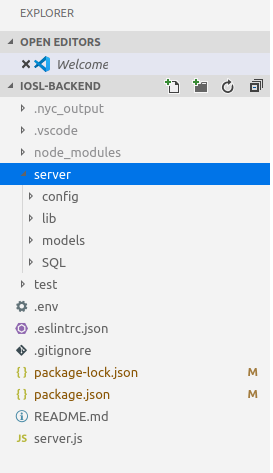
\includegraphics[width=4cm]{images/directystructure.png}
    \caption{Directory Structure}
    \label{fig:}
\end{figure}

\begin{itemize}

\item {\textbf{Server}}: This folder contains all the logic related to server functionality. 
\begin{itemize}
\item {\textbf{Config}}: This folder contains the configuration for the server side. authkeys.js does contain the secret keys used across the application for google social login and to generate the token for authorization. Passport.js contains the logic for google strategy. we can write another strategy in the same file as well e.g. github or local strategy. In future, When we are going to integreate the platform with different vendors, we will be using the local passport strategy using the vendor database. After that, route.js does contain all the routes for the application. any new routes needs to be registered in this file. Finally token.util.js contains utility functions to generate and send the token to the client back. It also exposes the method to generate the token which is used for mocked unit testing. 

\item {\textbf{lib}}: Library or lib folder does contain the middleware for our back-end application. Right now we have only one, secureMiddleware, to secure our API endpoints. It does check if access-token header is provided in rquest body, cookie or querystring and then decode it using our secret. If successful it will set the user profile on the request object, otherwise throw 401 response. 

\item {\textbf{models}}: Models folder does contain all the different models to fetch the data from database or block chain. Each file represent an entity in the system or a related database relation.  Furthermore, index.js file contains the references of all the models and is used almost everywhere in the system as single reference point for the models. 

\item {\textbf{SQL}}: SQL folder contains the database schema which can be used to deploy or create the database while setting up a project on a new machine. Additionally, it contains a schema file to generate the database diagram on dbdiagram.io as well. 
\end{itemize}


\item {\textbf{test}}: This folder contains all the unit tests. Each file contains the tests for the respective model file. Test does use mocha and chai frameworks.

\item {\textbf{env}}: .env is environment file to setup variables at the start of the project instead of reading from the config file, it will be read from the environment. This file is git ignored. It isn't used at the moment as we are reading db config from the db.js directly for now. 

\item {\textbf{eslintrc.json}}: ESlint configuration can be changed using this file. We are using Airbnb base syntax for our linting.  

\item {\textbf{gitignore}}: GitIgnore is used to tell git which files we don't want to store in the source control. 


\item {\textbf{package.json}}: This file contains all the configuration to setup the project. When we do npm install, it will read this file and install all the package on end user machine. It also contains the dev dependencies. We have different scripts configured to run e.g. running the server or run server in the debug mode, run linter. 

\item {\textbf{server.js}}: This is the starting file where our project starts. This file will bootstrap the application by configuring different modules, followed by loading the routes and then running the http server on specific ports. We also configure the express server, body parser (which parse the request body), cookie-parser, passport js and most importantly CORS to send cross origin requests.   

\end{itemize}

\subsection{Unit Testing}
We are using mocha framework for unit and integration testing in our project. Additionally we have used chai as an assertion framework for our tests. Each test has a title or test case description followed by request and expected results. A sample test is as follows

\begin{verbatim}
  /*
  * /GET company/id
  * Test the single company records from the database
  */
  it('It should GET single company', (done) => {
    chai.request(server)
      .get('/company/2')
      .end((err, res) => {
        res.should.have.status(200);
        res.body.should.be.a('array');
        res.body.length.should.be.eql(1);
        done();
      });
  });



\end{verbatim}

We used chai request to call the endpoint, set the access token for the secured endpoints, and then compare the results with  the expectation. We also have tests which will send different access token to validate the authorization of the endpoints e.g. postman can see only packages assigned to him and not all the packages or a customer cannot request a handover for a package. 
